\chapter{实现}
\label{cha:impl}

\section{性能模型}
\label{sec:impl_model}
    在上文\ref{ssec:model}中我们提到,我们建立性能模型的主要方法是测试不同输入参数下,操作的运行时间,然后对得到的数据进行分段插值。本节中,我将分别对各个操作的建模方法进行介绍。
    
    我们的实验平台如下:
    
    \begin{itemize}
        \setlength{\itemindent}{1em}
        \item CPU:2个8核Intel Xeon CPU(E5-2620 v4)
        \item RAM:256GB
        \item GPU:4块Nvidia GPU(Tesla V100),使用NVLink连接
        \item OS:Ubuntu 18.04.1 LTS
    \end{itemize}

\subsection{矩阵乘法}
\label{ssec:impl_matmul}
    首先是计时方式的选择。在矩阵乘法这个操作中,三种方式均可以在大部分情况下正常使用,我们对CPU、GPU分别进行讨论。
    在CPU上,数据较小时,TensorFlow Profiler不能获得矩阵乘法操作的运行时间,因此我们选择直接对会话进行计时。在GPU上,我们通过nvprof监视volta\_sgemm函数的运行时间,可以直接得到矩阵乘法操作的计算时间,避免数据传输的影响。因此,我们在CPU上使用会话计时,在GPU上使用nvprof直接监视的方式的获取运行时间数据。

    之后是参数的选择。矩阵乘法包含三个参数$ M $、$ N $、$ P $。
    
    我们首先考虑CPU的情况。
    
    如果直接使用$ M \times N \times P $作为参数,得到的性能数据如图\ref{fig:matmul_cpu_nmp}所示。我们可以看到,尽管整体趋势上,运行时间和$ N \times M \times P $为正比例关系,但是相同$ N \times M \times P $取值下,时间差距较大。最差情况下,相同取值下,最长时间将比最短时间长1.38倍,此时这个取值的数据相对标准偏差接近0.3。因此,$ N \times M \times P $不是一个好的参数取值。
    
    \begin{figure}[!htbp]
        \centering
        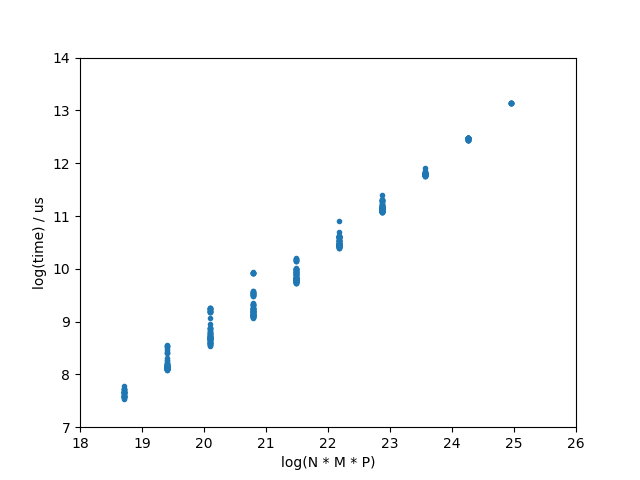
\includegraphics[width=0.8\textwidth]{figures/matmul_cpu_nmp.png}
        \caption{CPU矩阵乘法的性能数据(参数为$N \times M \times P $)}
        \label{fig:matmul_cpu_nmp}
    \end{figure}
    
    \begin{figure}[!htbp]
        \centering
        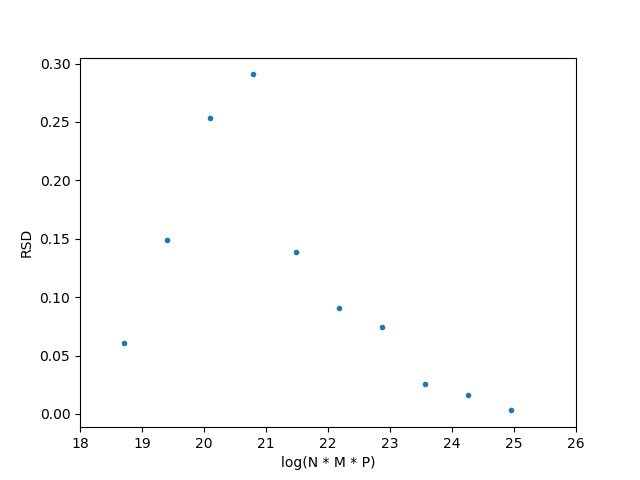
\includegraphics[width=0.8\textwidth]{figures/matmul_cpu_nmp_rsd.png}
        \caption{CPU矩阵乘法的相对标准偏差数据(参数为$ N \times M \times P $)}
        \label{fig:matmul_cpu_nmp_rsd}
    \end{figure}
    
    接下来我们考虑\ref{ssec:view_matmul}中提到的矩阵乘法计算过程,我们选取$ N \times M $和$ P $作为参数,这时我们发现数据相对$ N \times M $和$ P $都保持了比较好的正比例关系,同时,在固定参数取值的情况下,相对标准偏差低于0.1,可以满足我们的预测需求。因此,在CPU上最终的矩阵乘法性能模型采用$ N \times M $和$ P $作为参数,对性能数据进行线性插值。
    
    \begin{figure}[!htbp]
        \centering
        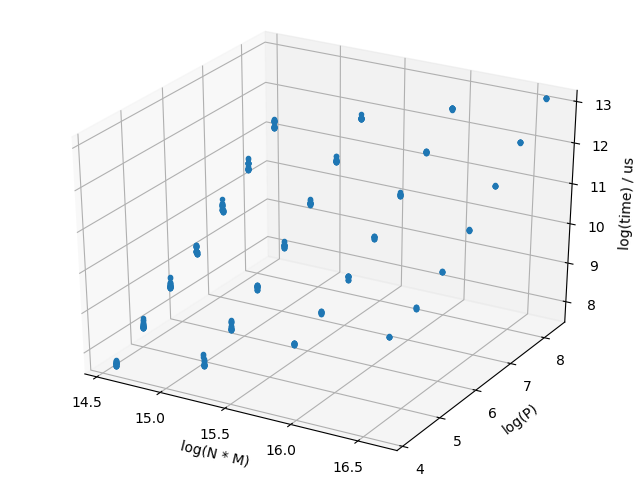
\includegraphics[width=0.8\textwidth]{figures/matmul_cpu_nm_p.png}
        \caption{CPU矩阵乘法的性能数据(参数为$N \times M $和$ P $)}
        \label{fig:matmul_cpu_nm_p}
    \end{figure}

    \begin{figure}[!htbp]
        \centering
        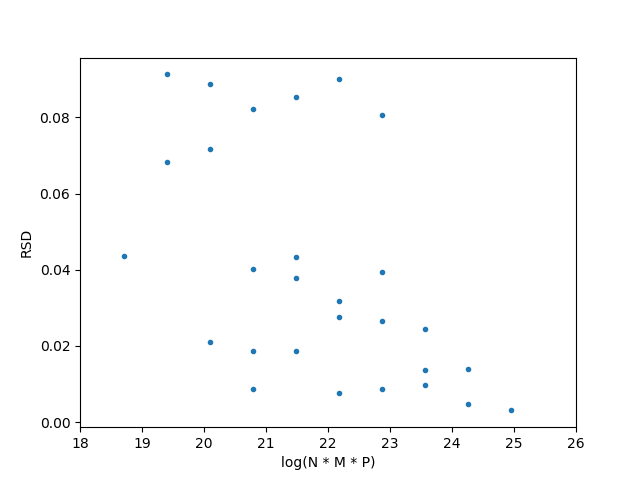
\includegraphics[width=0.8\textwidth]{figures/matmul_cpu_nm_p_rsd.png}
        \caption{CPU矩阵乘法的相对标准偏差数据(参数为$ N \times M $和$ P $)}
        \label{fig:matmul_cpu_nm_p_rsd}
    \end{figure}

    下面我们来对GPU数据进行建模。首先我们观察以$ N \times M \times P $为参数的数据,如图\ref{fig:matmul_gpu_nmp}所示。我们可以发现,在$ N \times M \times P $取值较大的时候,性能变化较少,而且很符合正比例函数。但是在取值较小的时候关系不明显,而且变化较大。
    
    我们考虑GPU计算矩阵乘法的过程,$ M \times N $代表线程数量,而GPU中线程数量和CPU相比大很多,以我们的实验平台NVIDIA Tesla V100为例,NVIDIA Tesla V100单卡支持线程数为5120,因此,在$ N \times M$规模不同的时候,显然矩阵乘法的时间模型会有所不同。这时我们对该模型进行分段,规模较小的数据,数据取值范围较小,我们直接使用$ M $、$ N $、$ P $作为参数进行建模。
    
    \begin{figure}[!htbp]
        \centering
        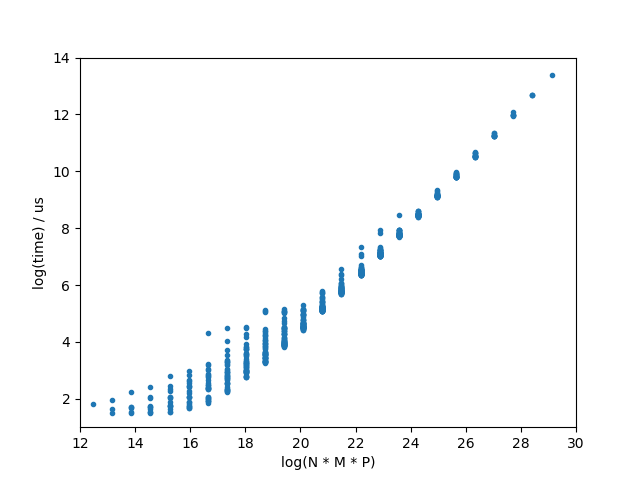
\includegraphics[width=0.8\textwidth]{figures/matmul_gpu_nmp.png}
        \caption{GPU矩阵乘法的性能数据(参数为$N \times M \times P $)}
        \label{fig:matmul_gpu_nmp}
    \end{figure}

    \begin{figure}[!htbp]
        \centering
        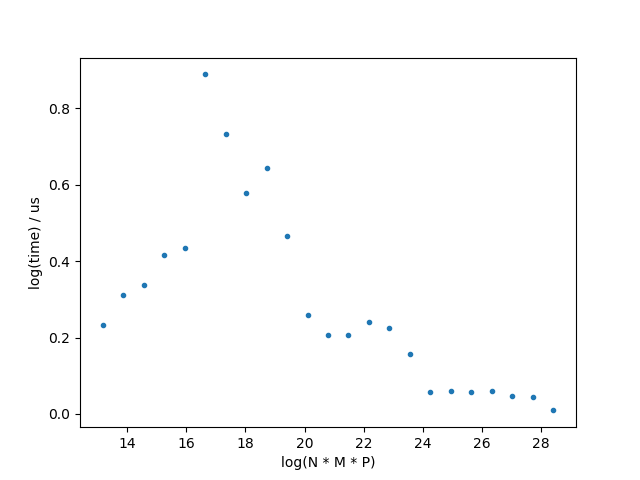
\includegraphics[width=0.8\textwidth]{figures/matmul_gpu_nmp_rsd.png}
        \caption{GPU矩阵乘法的相对标准偏差数据(参数为$ N \times M \times P $)}
        \label{fig:matmul_gpu_nmp_rsd}
    \end{figure}
    
    针对较大规模的数据,我们把$ N $、$ M $规模限制到128以上,性能数据如图\ref{fig:matmul_gpu_nmp_big}所示,我们可以看出,无论是数据的线性程度还是数据的变化范围都有了很大的提升。图\ref{fig:matmul_gpu_nmp_rsd_big}指出,从相对标准偏差值来看,相较图\ref{fig:matmul_gpu_nmp_rsd},在矩阵规模较大的时候,使用$ N \times M \times P $为参数,就可以达到比较好的预测效果了。
    
    \begin{figure}[!htbp]
        \centering
        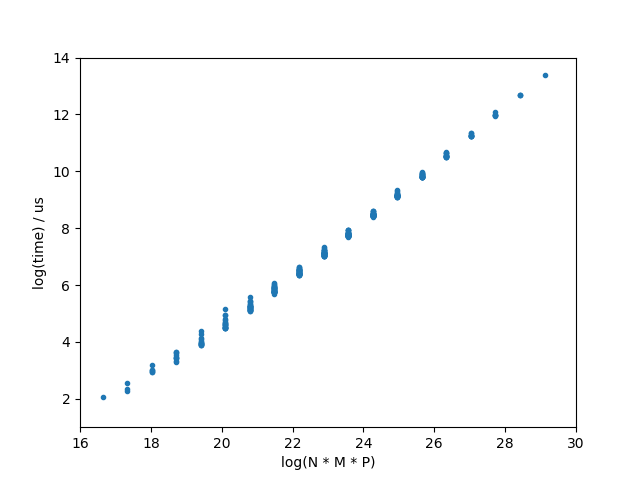
\includegraphics[width=0.8\textwidth]{figures/matmul_gpu_nmp_big.png}
        \caption{GPU矩阵乘法的性能数据(参数为$N \times M \times P $,$ N $、$ M $、$ P $取值128以上)}
        \label{fig:matmul_gpu_nmp_big}
    \end{figure}

    \begin{figure}[!htbp]
        \centering
        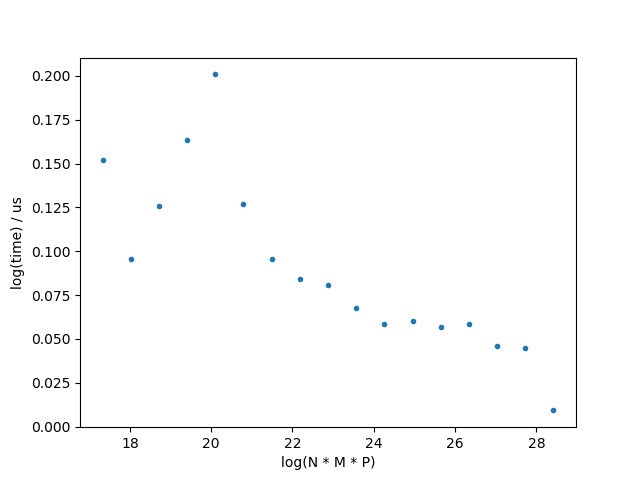
\includegraphics[width=0.8\textwidth]{figures/matmul_gpu_nmp_rsd_big.png}
        \caption{GPU矩阵乘法的相对标准偏差数据(参数为$ N \times M \times P $,$ N $、$ M $、$ P $取值128以上)}
        \label{fig:matmul_gpu_nmp_rsd_big}
    \end{figure}

    因此,我们将输入规模以128作为分界线,使用两个模型,小模型使用$ N $、$ M $、$ P $三个参数建模,而大模型使用$ N \times M \times P $作为参数建模,就能得到比较准确的预测结果了。

\subsection{二维卷积}
\label{ssec:impl_conv}
    二维卷积的操作计时过程较为复杂。首先,在CPU上,我们使用会话计时的方式进行测试。在GPU上,nvprof对一个卷积操作的统计过程中会追踪到多个CuDNN函数调用,此时针对这些函数进行分析是比较复杂的,同时也会带来更大的误差。但是同时,由于数据传输的存在,我们不能直接采用会话计时的方式。因此,我们通过nvprof统计数据传输时间,用会话计时减去数据传输,得到二维卷积操作的计算执行时间。

    在参数选择上,二维卷积操作的运算包含6个参数,图片数量($ B $)、图片尺寸($ W \times H $)、卷积核尺寸($ W_K \times H_K $)、输入通道数($ C_{in} $)、输出通道数($ C_{out} $)、步长($ W_S \times H_S $)。因此我们针对以上六个参数进行性能测试,得到在CPU和GPU上的性能数据。

    首先考虑CPU的情况,我们使用$ B \times W \times H \times W_K \times W_H \times W_S^{-1} \times H_S^{-1} \times C_{in} \times C_{out} $作为参数,得到性能数据如图\ref{fig:conv_cpu}所示。我们看到,参数取值相同时,数据变化范围较大,不能够直接使用。而我们经过观察,可以看出,性能数据图中隐约显示出4条平行的直线。而数据中取值有4种的参数仅有$ C_{in} $和$ C_{out} $,因此,我们取参数$ B \times W \times H \times W_K \times W_H \times W_S^{-1} \times H_S^{-1} \times C_{in} $和$ B \times W \times H \times W_K \times W_H \times W_S^{-1} \times H_S^{-1} \times C_{out} $。我们发现,当我们仅选$ B \times W \times H \times W_K \times W_H \times W_S^{-1} \times H_S^{-1} \times C_{in}  $为参数时图像变得较为清晰,如图\ref{fig:conv_cpu_fix0}所示。但依然有大量点不符合正比例函数。
    
    在二维卷积操作中,如果卷积核仅为一个点,那么二维卷积运算会退化为矩阵和数字的乘法,此时不会调用二维卷积操作的函数,因此,我们去除这类点,得到性能数据如图\ref{fig:conv_cpu_fix1}所示,此时平均相对标准偏差为0.18可以满足我们的需求。

    \begin{figure}[!htbp]
        \centering
        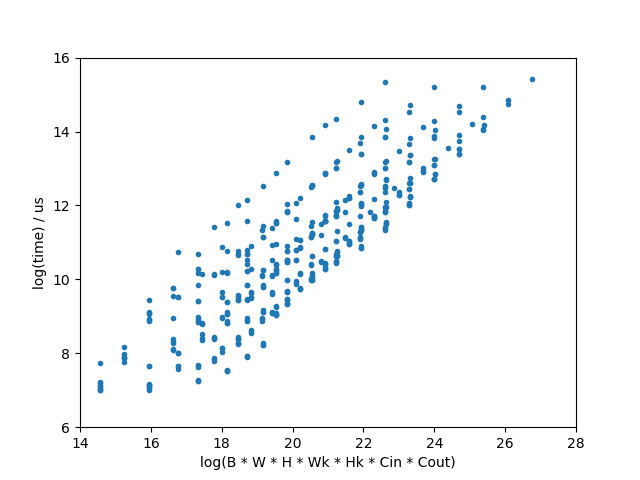
\includegraphics[width=0.8\textwidth]{figures/conv_cpu.png}
        \caption{CPU二维卷积的性能数据(参数为用$ B \times W \times H \times W_K \times W_H \times W_S^{-1} \times H_S^{-1} \times C_{in} \times C_{out} $)}
        \label{fig:conv_cpu}
    \end{figure}

    \begin{figure}[!htbp]
        \centering
        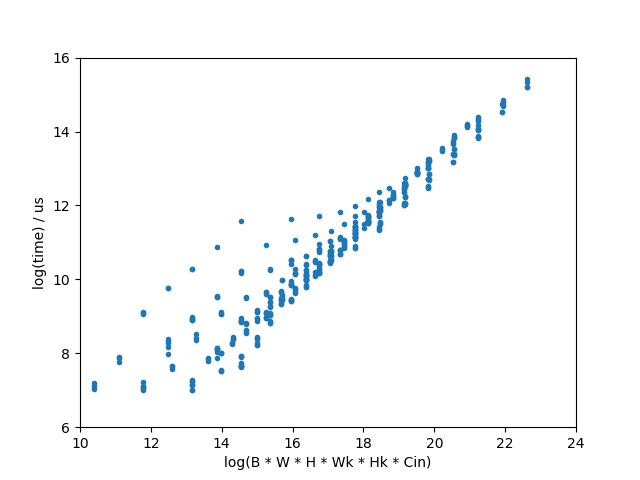
\includegraphics[width=0.8\textwidth]{figures/conv_cpu_fix0.png}
        \caption{CPU二维卷积的性能数据(参数为$ B \times W \times H \times W_K \times W_H \times W_S^{-1} \times H_S^{-1} \times C_{in}  $)}
        \label{fig:conv_cpu_fix0}
    \end{figure}

    \begin{figure}[!htbp]
        \centering
        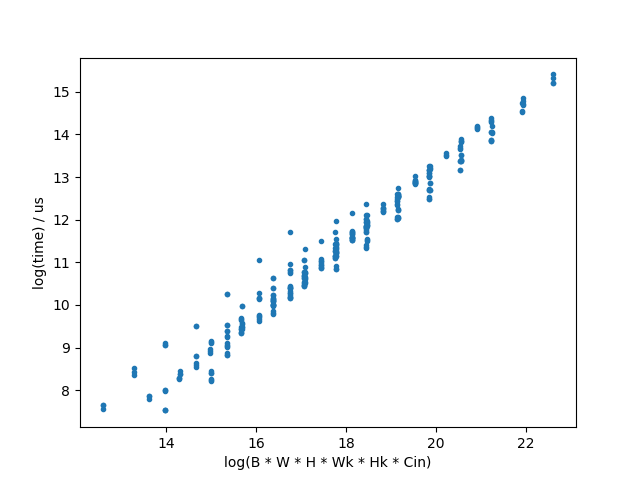
\includegraphics[width=0.8\textwidth]{figures/conv_cpu_fix1.png}
        \caption{CPU二维卷积的性能数据(参数为$ B \times W \times H \times W_K \times W_H \times W_S^{-1} \times H_S^{-1} \times C_{in}  $,去除卷积核大小为1的情况)}
        \label{fig:conv_cpu_fix1}
    \end{figure}

    在GPU上,二维卷积操作会采用不同的优化方式,调用不同的CuBlas或CuDNN函数,这时数据规律并不直观,因此我们无法直接降低参数个数,只能直接对数据进行插值。
    
    \begin{figure}[!htbp]
        \centering
        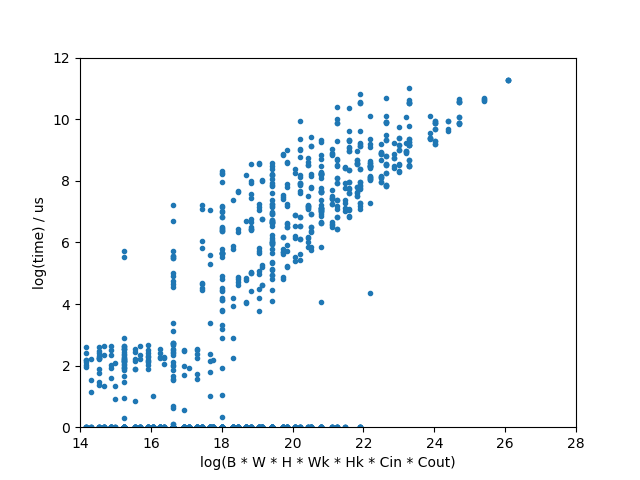
\includegraphics[width=0.8\textwidth]{figures/conv_gpu.png}
        \caption{GPU二维卷积的性能数据(参数为$ B \times I^2 \times K^2 \times C_{in} \times C_{out} $)}
        \label{fig:conv_gpu}
    \end{figure}
    
\subsection{局部响应归一化}
    局部响应归一化的操作计时较为简单。CPU上我们直接使用会话计时的方法进行。GPU上,该函数没有预先定义CuDNN或CuBlas函数对应,因此nvprof无法直接通过函数调用得到该操作的运行时间,因此采用会话计时减去数据传输时间的方式获得GPU上的运行时间。

    局部相应归一化的输入是一个四维张量。其中前三维的乘积我们作为参数$ M $,第四维作为参数$ N $,深度半径作为参数$ R $。

    在CPU上,我们以$ M \times N $为参数,这时局部响应归一化的性能数据如图\ref{fig:lrn_cpu}所示,此时的平均相对标准偏差为0.15可以满足我们的需求。
    
    \begin{figure}[!htbp]
        \centering
        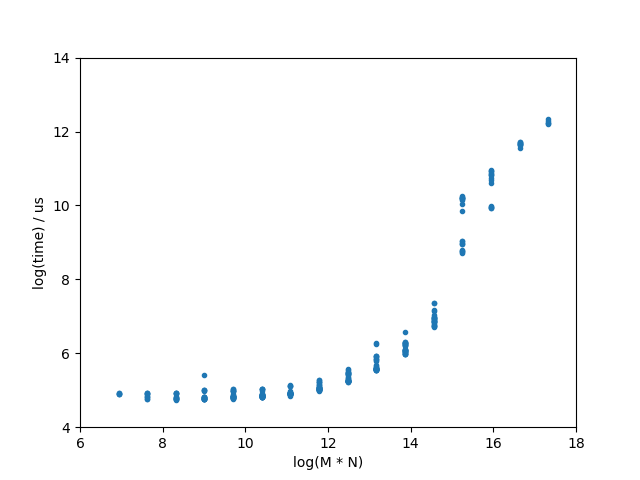
\includegraphics[width=0.8\textwidth]{figures/lrn_cpu.png}
        \caption{CPU局部响应归一化的性能数据(参数为$ M \times N $)}
        \label{fig:lrn_cpu}
    \end{figure}

    在GPU上,以$ M \times N $为参数,局部响应归一化函数的性能数据如图\ref{fig:lrn_gpu}所示,此时平均相对标准偏差为0.14,也满足我们的需求。

    \begin{figure}[!htbp]
        \centering
        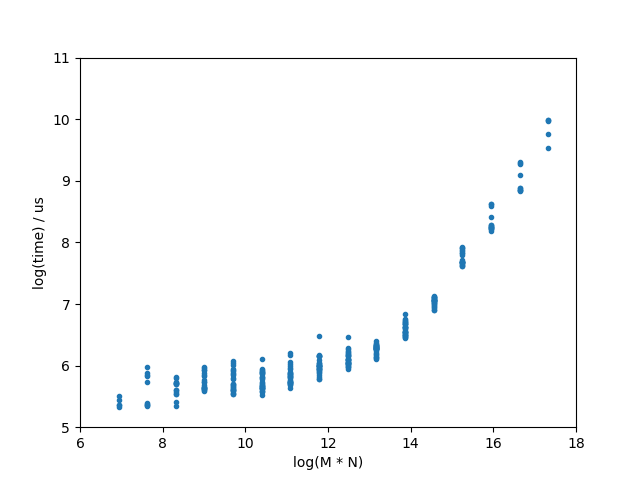
\includegraphics[width=0.8\textwidth]{figures/lrn_gpu.png}
        \caption{GPU局部响应归一化的性能数据(参数为$ M \times N $)}
        \label{fig:lrn_gpu}
    \end{figure}

\subsection{数据传输}
    在使用GPU的情况下,我们还需要考虑CPU和GPU之间,GPU和GPU之间的数据传输问题,即对cuMemcpyDtoH, cuMemcpyHtoD, cuMemcpyPtoP进行建模。
    我们默认TensorFlow能够占用整个机器的所有资源,不会和其他应用抢占。这时不考虑函数调用带来的时间,那么我们的数据传输能够占用所有的带宽。因此,cuMemcpyDtoH和cuMemcpyHtoD的执行时间应该为数据传输量除以PCIE带宽。而cuMemcpyPtoP的执行时间为数据传输量除以NVLink带宽。

    以我们的实验平台为例,PCIE带宽为32GB/s。我们直接建模。NVLink带宽为900GB/s,运行时间过快,不会对我们的模型造成影响,因此省略。

\subsection{数据修正}
    之前讨论的性能模型中,都存在不很符合我们预测模型的数据点,对这类数据点,我们采用提前存储的方式进行处理。针对之前测试中离模型相差过远的数据点,我们测试它周围一定范围的数据。测试数据落在这个范围内时,我们使用这一范围内的数据点进行插值,作为最终的预测结果,从而避免之前建立的模型精度不足的情况。
    
    另外,由于常用的卷积神经网络中使用的卷积操作规模都比较相似,因此,我们也可以将常用的操作参数也作为特殊点进行测试,这样在测试的时候,我们就可以更容易地得到准确的性能数据。在后续测试中,为了保证实验的可信性,我们没有在评价测试使用的版本中部署这个优化。

\section{调度模拟}
    调度模拟部分主要处理四部分工作:
    \begin{itemize}
        \setlength{\itemindent}{1em}
        \item {\bfseries 生成}:将用户输入的TensorFlow代码转化为数据流图的形式。
        \item {\bfseries 剪枝}:根据输入输出列表对数据流图进行剪枝,得到最小依赖集。
        \item {\bfseries 预测}:根据设定好的配置代入性能模型数据,预测性能。
        \item {\bfseries 模拟}:动态模拟模型运行状况。
    \end{itemize}
    
    下面分别就四部分工作的实现进行讲解。

\subsection{生成}
    数据流图的生成,我们通过直接调用TensorFlow接口的方式进行。用户正常编写TensorFlow代码,我们创建会话,获得计算图保存为JSON格式,作为下一部分的输入。

    接下来对计算图进行处理,首先根据JSON中的信息将图重新组织为点集的形式,每个点保存名称、输入、输出、操作类型等信息,再将用户输入的规模信息作为参数保存在相应节点上。最后将部分操作扩展为子图,即完成图的生成。

\subsection{剪枝}
    剪枝操作是为了获得最小依赖集,TensorFlow中使用DFS进行剪枝。在我们的系统中,结合我们的存储方式,我们使用BFS实现,从输出点开始,反向搜索依赖点,最终没有被覆盖的点直接删除。

    实际正常定义的深度神经网络任务中,不存在冗余节点,因此这一步并不能有效减少预测信息内容。

\subsection{预测}
    预测部分将每个操作需要的计算时间填入到数据流图中对应节点的信息中。由于操作执行的硬件信息被存储到了数据流图的节点中,因此这一步只需要遍历数据流图,查询性能模型,再写入数据即可。

\subsection{模拟}
    在得到准备好的数据流图后,我们进行调度模拟,以求尽量还原TensorFlow的动态调度过程。

    考虑到在二维卷积操作在CPU上可能存在的不能占满所有线程的情况。我们在模拟过程中还需要考虑每个任务在当前运行状态下,实际能占用的CPU计算资源比例。

    我们首先将输入节点加入待运行队列中,在每一轮运行时,我们根据资源使用情况,尽量将新的节点加入运行,每一轮运行的时候根据当前操作占用的资源调整每个操作的剩余时间,如原本操作占用所有CPU资源,还需要运行400ms,那么加入一个新的操作后,该操作只能占用50\%的资源,因此剩余时间变化为800ms。选择完成时间最短的操作,更新整体完成时间,再进入下一轮迭代。重复这一个过程,我们就可以比较准确地模拟TensorFlow中操作的动态调度过程了。

    实际使用中,由于性能模型存在误差,因此不能保证调度过程和TensorFlow的调度过程完全相同。但是考虑到一般的卷积神经网络是分层的,层间还有同步,因此我们的预测模式在调度层面通常不会带来很大的误差,这一点在\ref{cha:eval}中会详细介绍。
